\documentclass[margin=2mm]{standalone}
%\usepackage{bm}
%\usepackage{calligra}
\usepackage{amsmath} % assumes amsmath package installed
\usepackage{amssymb}  % assumes amsmath package installed
\newcommand{\setfont}[2]{{\fontfamily{#1}\selectfont #2}}
\usepackage{tikz}
\usepackage{pgfplots}
\usetikzlibrary{3d}

\usetikzlibrary{calc}
\usetikzlibrary{patterns}
\usetikzlibrary{decorations.text}
\usetikzlibrary{decorations.pathmorphing}
\usetikzlibrary{decorations.markings}
\usetikzlibrary{arrows}
\usetikzlibrary{shapes}

\pgfdeclareimage[width=2.0cm]{VectorFields}{EllipseBetaThird}

\newcommand{\picturefontsize}{\LARGE}
\newcommand{\pictureLineWidth}{0.8mm}

\begin{document}
%!TEX root = ../../14-icra-RealTimeNMPC.tex

\newcommand{\tetazero}{20.55}
\newcommand{\Fkxzero}{-20}
\newcommand{\Fkyzero}{20}

\newcommand{\tetaone}{-20}
\newcommand{\Fkxone}{5}
\newcommand{\Fkyone}{0}

\newcommand{\tetatwo}{20}
\newcommand{\Fkxtwo}{25}
\newcommand{\Fkytwo}{20}


\definecolor{txtcolor1}{RGB}{1, 121, 111}% corail
\definecolor{txtcolor2}{RGB}{27, 79, 8}% orange 
\definecolor{txtcolor3}{RGB}{237 , 127 ,16}%
\definecolor{txtcolor4}{rgb}{0.9,0.,0.}


%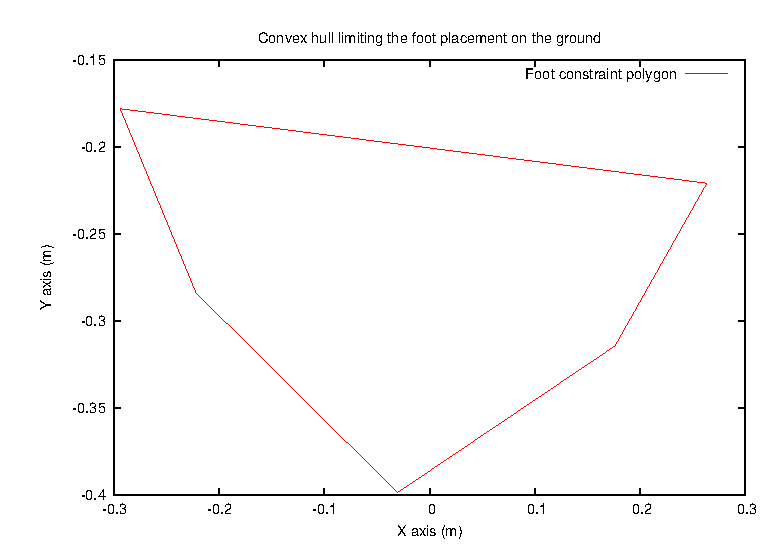
\includegraphics[width=15cm]{./figures/walking-without-thinking/ConvexHull}
\begin{tikzpicture}
\begin{axis}
%[hide axis]
[xlabel=x,ylabel=y]
\addplot[dashed,black,thick=2pt,fill=gray!20] table{foot.dat};
\addplot[black,thick=5pt,fill=gray!20] table{footconstraint.dat}; 
\addplot[black,thick=2pt,fill=gray!20] table{footmargin.dat};
\addplot[txtcolor1,thick=2pt] table[x index= 0,y index=1] {table.dat}; 
\addplot[txtcolor2,thick=5pt] table[x index= 2,y index=3] {table.dat}; 
\end{axis}
\shade[ball color=gray] (4.25,5) circle (0.6cm);
\draw [line width=2pt,red](2.5,5.2)--(6.5,3.2) node at (2.5,6.0)[red]{additional linear constraint} ;

\end{tikzpicture}

\end{document}
